\documentclass[tikz,border=8pt]{standalone}
\usepackage{amsmath}
\usepackage{newtxtext,newtxmath}
\usetikzlibrary{arrows.meta,positioning,fit,backgrounds,calc,
  decorations.pathmorphing}

\definecolor{ink}{HTML}{1B2A38}
\definecolor{acc}{HTML}{0A8F9E}
\definecolor{accfill}{HTML}{E7F4F5}
\definecolor{grayfill}{HTML}{EEF1F4}
\definecolor{line}{HTML}{C7D2DA}
\definecolor{good}{HTML}{0F9D76}
\definecolor{bad}{HTML}{C24A3B}
\definecolor{cdelta}{HTML}{3B5BD0}\definecolor{ctheta}{HTML}{6741C9}
\definecolor{calpha}{HTML}{0F9D76}\definecolor{cbeta}{HTML}{D18A00}
\definecolor{cgamma}{HTML}{D1541F}

\begin{document}
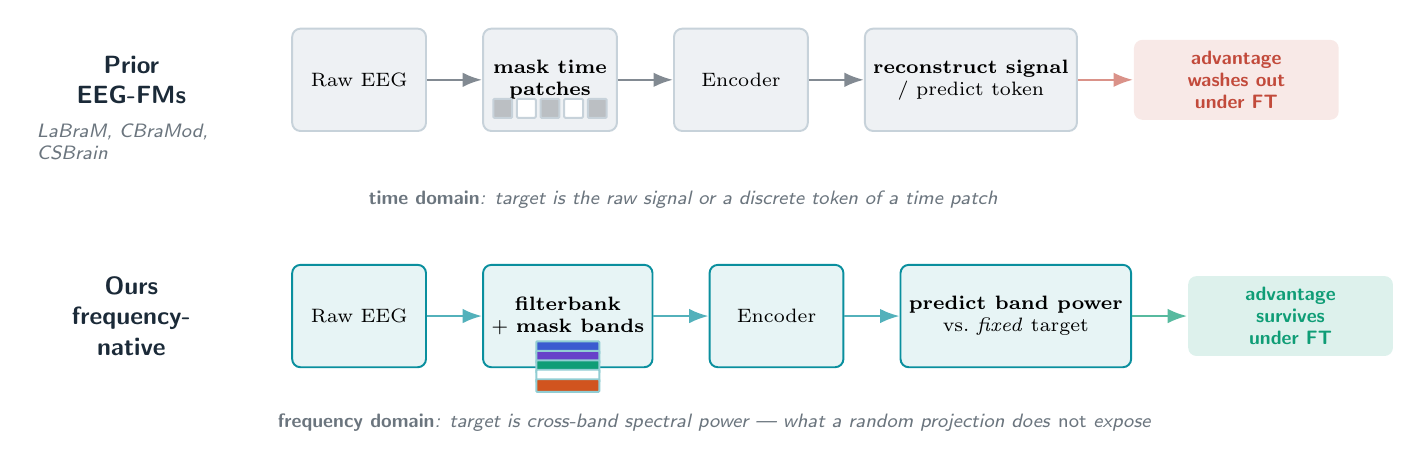
\begin{tikzpicture}[font=\sffamily,>=Latex,line width=.7pt,
  b/.style={draw=line,rounded corners=3pt,minimum height=13mm,minimum width=17mm,
    align=center,inner sep=3pt,font=\scriptsize},
  rowlbl/.style={align=center,font=\sffamily\small\bfseries,text=ink},
  flow/.style={->,draw=ink!55,line width=.9pt},
  capt/.style={font=\sffamily\scriptsize\itshape,text=ink!65},
  outcome/.style={rounded corners=3pt,align=center,font=\sffamily\scriptsize\bfseries,
    inner sep=4pt,minimum width=26mm}]

% ============ ROW 1 : PRIOR (time-domain) ============
\begin{scope}[local bounding box=row1]
 \node[rowlbl,text width=22mm] (p0) {Prior\\EEG-FMs};
 \node[capt,below=0pt of p0,text width=24mm] {LaBraM, CBraMod, CSBrain};
 \node[b,fill=grayfill,right=8mm of p0] (p1) {Raw EEG};
 % masked TIME patches
 \node[b,fill=grayfill,right=7mm of p1] (p2)
   {\textbf{mask time}\\\textbf{patches}};
 \foreach \i/\f in {0/ink!30,1/white,2/ink!30,3/white,4/ink!30}{
   \node[minimum size=2.4mm,inner sep=0,rounded corners=.4pt,fill=\f,draw=line]
     at ($(p2.south)+({(\i-2)*3mm},3mm)$){};}
 \node[b,fill=grayfill,right=7mm of p2] (p3) {Encoder};
 \node[b,fill=grayfill,right=7mm of p3,minimum width=24mm] (p4)
   {\textbf{reconstruct signal}\\/ predict token};
 \foreach \a/\b in {p1/p2,p2/p3,p3/p4}\draw[flow] (\a)--(\b);
 \node[outcome,fill=bad!12,text=bad,right=7mm of p4] (o1)
   {advantage\\ washes out\\ under FT};
 \draw[flow,draw=bad!60] (p4)--(o1);
\end{scope}
\node[capt,below=1.5mm of row1] {\textbf{time domain}: target is the raw signal or a
  discrete token of a time patch};

% ============ ROW 2 : OURS (frequency-domain) ============
\begin{scope}[local bounding box=row2,shift={(0,-30mm)}]
 \node[rowlbl,text width=22mm] (q0) {\textbf{Ours}\\frequency-\\native};
 \node[b,fill=accfill,right=8mm of q0,draw=acc] (q1) {Raw EEG};
 % filterbank bands
 \node[b,fill=accfill,right=7mm of q1,draw=acc] (q2)
   {\textbf{filterbank}\\+ \textbf{mask bands}};
 \foreach \f/\i in {cdelta/0,ctheta/1,calpha/2,white/3,cgamma/4}{
   \node[minimum width=8mm,minimum height=1.6mm,inner sep=0,rounded corners=.3pt,
     fill=\f,draw=acc!45]
     at ($(q2.south)+(0,{2.6mm-\i*1.2mm})$){};}
 \node[b,fill=accfill,right=7mm of q2,draw=acc] (q3) {Encoder};
 \node[b,fill=accfill,right=7mm of q3,minimum width=24mm,draw=acc] (q4)
   {\textbf{predict band power}\\{\scriptsize vs.\ \emph{fixed} target}};
 \foreach \a/\b in {q1/q2,q2/q3,q3/q4}\draw[flow,draw=acc!70] (\a)--(\b);
 \node[outcome,fill=good!14,text=good,right=7mm of q4] (o2)
   {advantage\\ \textbf{survives}\\ under FT};
 \draw[flow,draw=good!70] (q4)--(o2);
\end{scope}
\node[capt,below=1.5mm of row2] {\textbf{frequency domain}: target is cross-band
  spectral power --- what a random projection does \emph{not} expose};

\end{tikzpicture}
\end{document}
